\subsection{Milestone}
Der \gls{Milestone} von GitHub entspricht dem Meilenstein im Kontext des
Projektmanagements.

\subsubsection{Title}
Der \gls{Title} entpricht der Identifikation und Kurzbeschreibung des
Meilensteins. Dieser gibt kurz und knapp Auskunft darüber, welcher
Projektfortschritt damit erreicht wird.

\subsubsection{Description}
Die \gls{Description} gibt eine detailliertere Beschreibung des Meilensteins
wieder. Diese enthält konkretere Angaben zum Inhalt und den Zielen des
Meilensteins.

\subsubsection{Due Date}
Der \gls{Due Date} gibt einen Termin an, in Form eines Datums, welcher das
Kontroll- oder Fälligkeitsdatum eines Meilensteins darstellt.

\subsubsection{Status}
Der Status eines Meilensteins wird auf dem Webinterface von GitHub in einem
Balken dargestellt. Dieser stellt das prozentuale Verhältnis von
abgeschlossenen und ausstehenden Arbeitspaketen dar\footnote{Github kennt
keine Gewichtung von Arbeitspaketen.}. Die Abbildung
\ref{fig:milestone_progress} zeigt den abgeschlossenen
\gls{Milestone} \emph{Freigabe Gesamtkonzept, Projektdokumentation (80\%)}.
\begin{figure}[h!]
	\centering
	
\includegraphics[width=0.75\textwidth]{../../fig/github/milestone_progress.png}
	\caption{Status eines Meilensteins von \url{github.com/accefa/doku}}
	\label{fig:milestone_progress}
\end{figure}

Auf der Linken Seite ist der \gls{Title} dargestellt, darunterliegend das
Erfüllungsdatum (17. Dezember 2014) und das Datum der letzten Aktualisierung
(vor zwei Tagen). Auf der rechten Seite ist der Statusbalken (grün) zu
erkennen. Darunterliegend die Angabe in Prozent zum Status (100\%) und den
aktuellen Stand der zugehörigen \gls{Issue} (0 offen, 40 geschlossen).

\subsubsection{Zeitplan mit Meilensteinen}
Die erstellten Meilensteine können interaktiv in einem Browser betrachtet
werden. Diese sind in einer Übersicht eingefügt wie in Abbildung
\ref{fig:milestones} dargestellt. Die dargestellten Meilensteine führen per
Link auf die GitHub-Seite mit der Übersicht der Arbeitspakete zum
entpsrechenden Meilenstein.

\begin{figure}[h!]
	\centering
	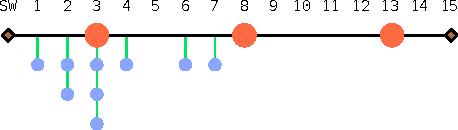
\includegraphics[width=0.5\textwidth]{../../fig/github/milestones.pdf}
	\caption{\href{github.com/accefa/}{Zeitstrahl mit eingetragenen Meilensteinen}}
	\label{fig:milestones}
\end{figure}
